% Chapter 1

\chapter{Introduction}

\label{chap:introduction} 

\graphicspath{{Figures/Introduction}}

Programming languages are media through which we communicate with machines our ideas, be it mathmatical formulae, or video games. Like human language, programming languages consists of words, grammar, and meaning. Unlike conversing with human, machines tolerate very little ambiguity and are not skillful at navigitting confusion. In this chapter we inspect two spectrum of programming language design: their typing discipline and the paradigm they reside. Through this we hope to illustrate a common pattern: the more certainty we get knowing our program run correctly, the more we are bothered with conforming to rules and checks. And when these rules and checks are violeted, when we meet the anguish of compiler in arcane jargons all in uppcase letters. My interventions aim to transform the error messages into clear diagnosis, assisted by interactive user interface to provide clarity, intuitiveness, and resolution.   


\section{From types to program correctness}

In programming language theory and practice, typing is a widely adopted program validation method where types of expressions are checked against their usage. From early stage of pragramming, types are used to inform compiler how much memory needs to be allocated for each value. Now days, types are wildly more powerful, programmers can express complex ideas, like commnication protocals, concurrency characteristics. Conventionally, the discipline of typing is identified by the existence of compile time checking stage. Program language is said to be statically typed if it check time before a program is executed.  On the other hand, dynamimcally typed languages (colloquially called dynamic languages) will not complain about type mismatch, and they do not facilitae the action of describing the types, and will result in a runtime error if such mismatch is not handled. Statically typed languages have a long history and are extremely popular, with examples of among both the earliest of programming languages (such as FORTRAN and ALGOL, \cite{Backus1978-xt}) and the most widely used languages across all platforms  (such as C and its derivatives including Java and C\#, \cite{Ritchie1978-pa}). Static typing is also a core feature of the most advanced and renowned academic languages (such as ML, Haskell, and their derivatives, such as OCaML and Agda, respectively, \cite{Hudak2007-kn}). In practice, statically typed programming languages offer many advantages. Type declarations and annotations add important contextual information about the expected use of variables and expressions. This additional context allows early error detection but also enhances code readability and promotes maintainability, especially in large collaborative projects. The explicit encapsulation of type information in code also creates opportunities for improved tooling through intelligent compiler services and IDE (interactive development environment) support. Additionally, static typing enhances the library documentation by providing clear contracts between library authors and users.


Compared to static typing, its – dynamic typing – provides many appealing benefits, and has strong influence in the computing world. In dynamically typed languages, a variable can hold different types of values because the type is checked during runtime. This provides more flexibility than static typing since a single variable can be used to hold different types of values through mutation or reassignment. However, it also means that errors such as trying to subtract a string from a number can be detected only when the code is run, leading to potentially dire concequeces. The lisp programming languages, such as common lisp and scheme, were designed to benefit from the flexibility of dynamic typing. In Lisp languages, functions often take dynamic input that can be various forms (atom, lists, s-expressions), and different code is executed based on inspecting the input value at runtime. In modern day computing,  languages like JavasScript, Python are all dynamic languages, which is believed to contribute to their immense popularity thanks to the lower barrier of entry.

\begin{figure}[hbt]
  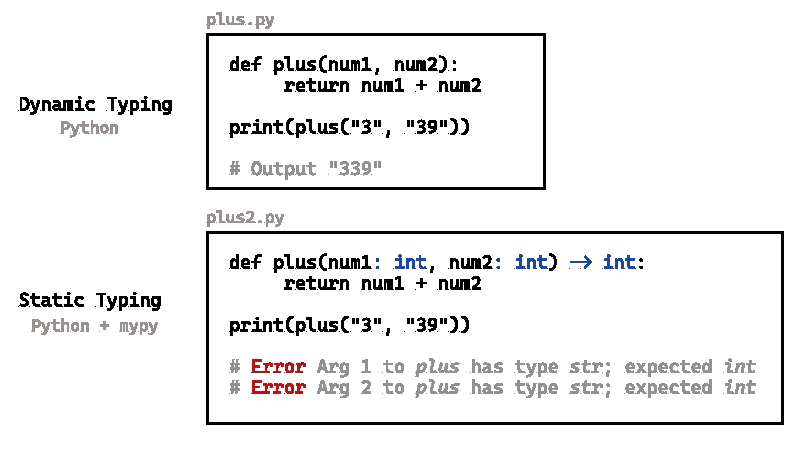
\includegraphics[width=\linewidth]{TypedVsUntyped.pdf}
  \caption{
    \label{fig:typed-vs-untyped}
   The same prgram that is dynamically typed in python (Top) and statically typed in python and mypy (Bottom).
    }
\end{figure}

It comes as no supprise that large amount of work were dedicated to decide which one of the two typing discipline is superior. Unfortunately not only these work failed to aggree on which one is better, nor do they aggree on how to define what is good. Nevertheless, the lessions from these work should not be discounted.  


\section{Functional Programming}
Of course, static typing is not the only techinuqe that embrace rigor and formalism. \textbf{Functional languages}, originated from lambda calculus as a foundation of mathematics in the 1930, promotes the idea of using functions as the fundamental building blocks of programming and developing abstractions by composing functions. 
More importantly, so-called `pure' functional programming languages adopt additional rigor from mathematics, such as immutable values (values can not be modified once declared) and referential transparency (functions will always produce the same output when given the same input).  Like static typing, functional language concepts help programmers avoid certain undesired behaviors, by removing or carefully separating the effectful computation from the pure transformation of input and output.
For instance, becasue of the removal of pointers and share memeory,  misaligned pointers and race conditions are essentially elimitated.
Thus, programs written in these languages can be safely tested and reasoned about, and it takes away the fear that program behavior can be disrupted by external uncertainties, such as network connections or even dates. 

Functional programming has been advocated as an ideal introductory to programming language. Functional programming advocates argue that it promotes mathmatical thinking and it enforce strict programming discipline (such as seperating data and transformation). 

\begin{figure}[hbt]
  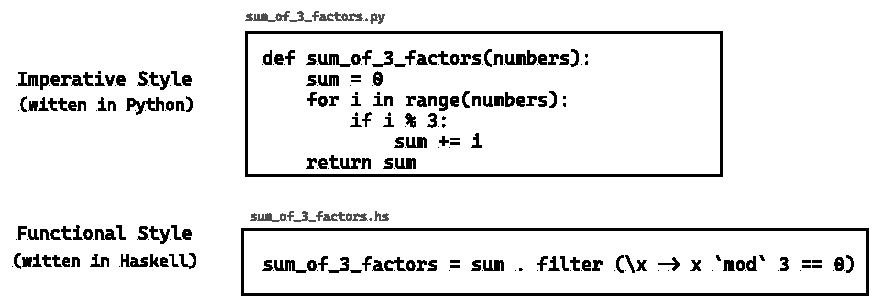
\includegraphics[width=\linewidth]{ImperativeFunctional}
  \caption{
    \label{fig:imperative-vs-functional}
   The same task of summing the factors of 3 in the given numbers, written in imparative style (Top) and functional style (Bottom).
    }
\end{figure}
Other paradigm of programming include object-oriented (where programs are orgnized by objects, within which data and behavior co-habit), and procedure programming (where programs are writen by specify a series a steps). In today's programming industry, other paradigm, object-oriented languages and procedure languages are still more popular than functional languages. At least, the traditional long serving languages, such as C and Java, appear to be more commertailly successful than any functional languages. And thus they are attracting new software projects to continue depend on them for the existing 3rd party library support and familiarity of tools.  Additionally, they often are able to provide a set of low level programming semantics that are close to the hardware. In C, pointers, locks, memory allocation are common concepts in these languages, that support programs written in these languages to be more efficient and performant. Lastly, the strictness in functional programming languages may raise the barrier to entry for beginners. For example, in many pure function languages, printing to the terminal window, a most common technique to observe the programs execution, require programmers to understand deep concepts like monad and side effects.  


\section{Statically Typed Functional Languages, The Best Of Both Worlds}
Combining the two disciplines, \textbf{statically typed functional languages} employ both static typing and the principles of functional programming. Most common statically typed function languages include Haskell,  ML (with the OCaml dialect being the most popular among the family of ML languages), and F\#. Languages like Idris and Agda even include more advanced type-level features like dependent type and session, allowing programmers to express granular checks of potential software behavior before running the program. These languages often provide the strongest level of programming safety. It is often advertised that programs in these languages will be error-free if the source code passes the compiling stage, indicating that compilers are able to weed out a large number of programming errors. These safety properties allow statically typed functional languages to be used as proof assistants or formal verification tools. They prove the correctness (or incorrectness) of many systems, from web public key infrastructure \cite{Bhargavan2021-no} to microcontrollers used in space programs \cite{Mokhov2019-zj}. Despite these safety benefits, these languages' presence in the mainstream programming world remains underwhelming. This lack of popularity is often attributed to higher barriers to entry, unfamiliarity, and unforgiving type errors.

\section{Symptoms of Bad Type Errors}
\ref{sec:symptoms}
 Compiler is the media programmers directly interact with to convert human intention into machine instructions. When encountering errors, compilers often ack like oracle, dishing out obsucre messages that often lead to huge confusion and wrong course of action. Many studies have investigated the ineffectiveness of compiler error messages \cite{}. In this we are more focused on type erros. The symptoms of common type error include:



 \subsection{Bias in Type Errors} 
 \label{subsec:bias}
 Bias in type error is when a type error can be caused by either one of multiple sources, but the type error only report one of them. This limitation has been known as left-to-right bias and has been often criticised \cite{McAdam2002-vb, Lee1998-fx, Chen2014-ev}. Left-to-right bias is a fundamental limitation of the traditional type checking algorithm, which we will revisit with greater details in Chapter \ref{chap:haskell-type-checking}. In the example in Fig \ref{fig:type-error-example}, it is more likely that the programmer is intend to compute the sum the two input numbers using the addition function \texttt{+} rather than concatenating the two inputs using the concatenation function \texttt{++}. However, the type error shows only one error suggesting that the function \texttt{addTwoNumbers} is given the wrong type of argument. 

 \begin{figure}[hbt]
  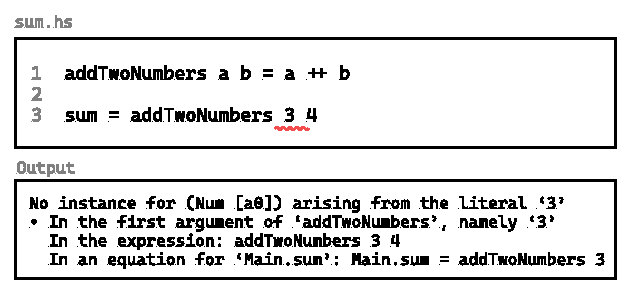
\includegraphics[width=\linewidth]{TypeErrorExample}
  \caption{
    \label{fig:type-error-example}
  In this example, programmer is likely misused the concatenation function \texttt{++} rather than addition \texttt{+} on line 1. However, the compiler will report that the error is the application of the interger literal \texttt{3}.
    }
\end{figure}


\subsection{Type Error Suggests Imcomplete Cause}
\label{subsec:imcomplete}

Type errors messages often show an imcomplete cause, meaning that fixing the higlighted location alone is not sufficient to resolve the type error. In the example in \ref{fig:type-error-example-2}, suppose that the programmer intend to write the function to concanate two lists, but applied the function with 2 interger value. However, in the type error, only the first argument is reported as an offending code, the second argument is spared. Programmer changing the literal \texttt{3} to \texttt{[3]} is not enough to make the type error go away, only updated to a slightly different error message. 


\begin{figure}[hbt]
  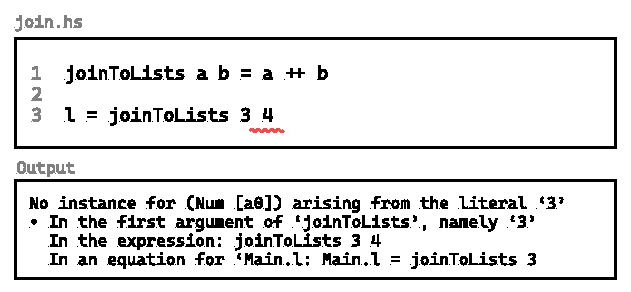
\includegraphics[width=\linewidth]{TypeErrorExample2}
  \caption{
    \label{fig:type-error-example-2}
  In this example, programmer is likely misused the concatenation function \texttt{++} rather than addition \texttt{+} on line 1. However, the compiler will report that the error is the application of the interger literal \texttt{3}.
    }
\end{figure}

\subsection{Missing Links In Type Errors}
\label{subsec:missing-link}

One of the most frustrating aspect of type error is that they do not show the complete steps of how it arrive at the conclusion. In the example in Fig \ref{fig:type-error-example-3}  programmer may intend to compare to a char literal \texttt{' '} instead of string literal \texttt{" "}. However, there are multiple clues in this code fragment: the definitaion of function \texttt{trimWhiteSpace}, the application of \texttt{filter isSpace a}, the definitaion of \texttt{isSpace}, and even the type signature of \texttt{filter} are all needed to understand how the error happens. In addition, these cluses need to be read in the logical order (not necessarily ordered by their appearance in the sourced) that support natual comprehension. 


\begin{figure}[hbt]
  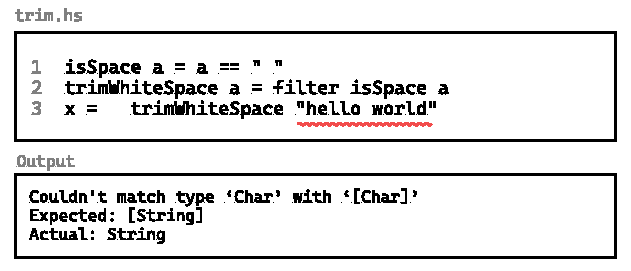
\includegraphics[width=\linewidth]{TypeErrorExample3}
  \caption{
    \label{fig:type-error-example-3}
  In this example, programmer may intend to compare to a char literal \texttt{' '} instead of string literal \texttt{" "}. However, the type error ignores all the important clues of how this error is inferred. 
    }
\end{figure}


\subsection{Language}

One that often upset beginners the most is that type erors are often full of tenical jargons or awewardly phrased. We have seen the common error such as \texttt{No instance for (Num a) arising from the literal `3'} which essentially means a char typed value is used at a place where a number type is requried."Error messages appear to take the form of natural language, yet are as difficult to read as source code". This bad design of type error messages are not unique to Haskell. In fact, this is often the common behavior in all programming language, and has been shown in many studies \cite{Barik2017-gy, Tirronen2015-nr, Prather2017-dg}. Many studies have sought to improve programmers' ability to solve errors by rephrasing the error message in the way that support understanding \cite{Becker2016-kc,Barik2014-ib} all show positive results.


\section{The Open Challenges Of Making Good Type Errors}

One major issue stemming from the promises of statically typed languages is the complexity involved in the systems and tools that safeguard the type-checking process. Ordinarily, this complexity is hidden away from the users. However, most compiler tools fail in usability when they encounter incorrectly typed programs. Type errors can be notoriously difficult to understand and use, particularly for newcomers to programming or when using a language that is particularly strict about types. Type errors are often believed to be a major contributor to static typing's reputation of being a high barrier to entry. I believe it is important to understand the root of the challenges of using type errors in order to address them. To achieve that, I believe it is useful to put type errors in proper context, more specifically, comparing them with other classes of programming errors (parsing errors, runtime errors). 

\subsection{Types Are As Complex As Runtime Values}
A major issue that many researchers, language designers and tool makers often overlook (or neglect) is types are very complex. In languages that implement dependent types, types are natually programs. Despite the fact that types are only computed at compile time, the computation that can happen are just as complex. Even in many programming languages that are dependently typed, type checking is shown to be non-terminating and Turing complete~\cite{Wells1999-ob}. For instance, in TypeScript the contintional types allow  This raises the challenge of explaining such a complex computing process when programmers are burdened to correct ill-typed programs. 


\begin{figure}[hbt]
  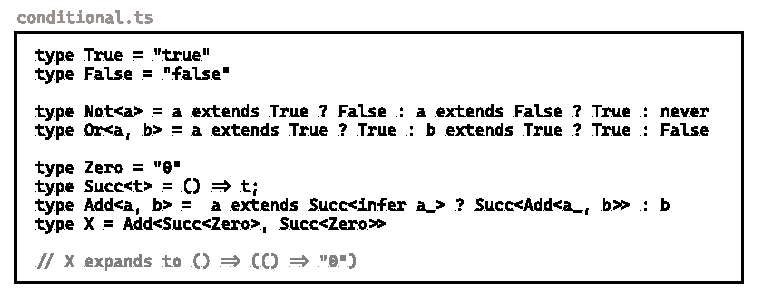
\includegraphics[width=\linewidth]{Conditional}
  \caption{
    \label{fig:conditional}
   TypeScript introduced a feature called conditional types, allowing programmers to write complex logic in type level. This will allow type annotation to be as complex as the program it descirbe.
    }
\end{figure}

\subsection{Clues For Type Checking May Be Implicit}
Understanding how types are assigned in a program becomes more challenging when the programming language uses type inference. Type inference \cite{Damas1982-sc},  also known as implicit typing, is a technique that allows programmers to omit the ritual of writing type annotations altogether, and the type checker will infer the most general types (principal types) for each expression. Even for languages that don't employ implicit typing, some typing rules are hidden from programmers.
For example, different programming language has its own rule of what can be compared by the \texttt{==} operator. In programming languages that have a record data type, programmers are burdened to consider adding an extra field or removing a filed still type correct or not \ref{fig:row-polymophism}, often taking into account the language specific rules such as covariance, contravriance, and subsumption.

\begin{figure}[hbt]
  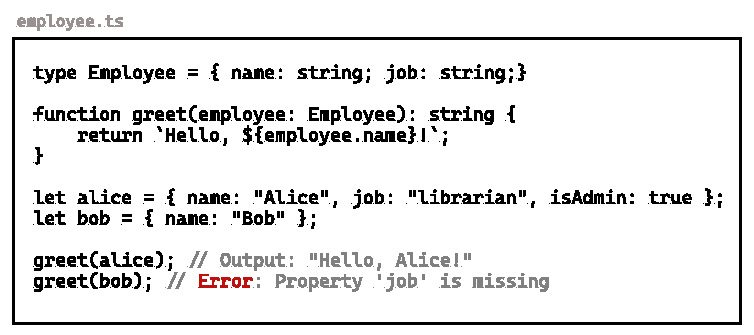
\includegraphics[width=\linewidth]{RowPolymorphism.pdf}
  \caption{
    \label{fig:row-polymophism}
   In many languages support row-polymophism, programmers enjoy more freedom in the fields of a data collection,  depending on situation,  extra fields or missing fields are allowed. However the rule of subsumptions (which type can substitute another type) are also obsecured.
    }
\end{figure}


\subsection{Lack of tool support}
Debugging programming errors have been an essential part of programming since the begining of computing, dating back as early as 1949 \cite{Campbell-Kelly1992-rn}. 

The simplest and most reliable appraoch is to inserting \texttt{print} statement. "The most effective debugging tool is careful thoughht coupled with judiciously placed print statements", computing pioneer Brian W. Kernighan \cite{Kernighan1978-xs}.  In addition, breakpoint debugging are very common debugging methods that have been integreated into almost all programming IDEs \ref{fig:breakpoint}. Moreover, research in the area of supporting error debugging has been very active. ZStep94 \cite{Lieberman1995-lg} extend the idea of breakpoint debugging, without the needs to add any breakpoint, allowing prorgammers to see all the historical values assumed by an expression. It also allows programemrs to incrementally navtigate forward and backword in execution history. WhyLine \cite{Ko2009-uf} is an Java program IDE that embrace the idea of natual programming environment \cite{Myers2004-fy}. It allows programmers to ask question in the program about why certain variable does not have the expected value. 

However the develoment type debugging has frozen in time, as most programming languages and develoment environments present type error the same manner as FORTAN and ALGO. Recent years, a few languages, such as Elm and Rust, have taking actions to improve type errors. Unfortunately, the changes they have made are superfacial.

\begin{figure}[hbt]
  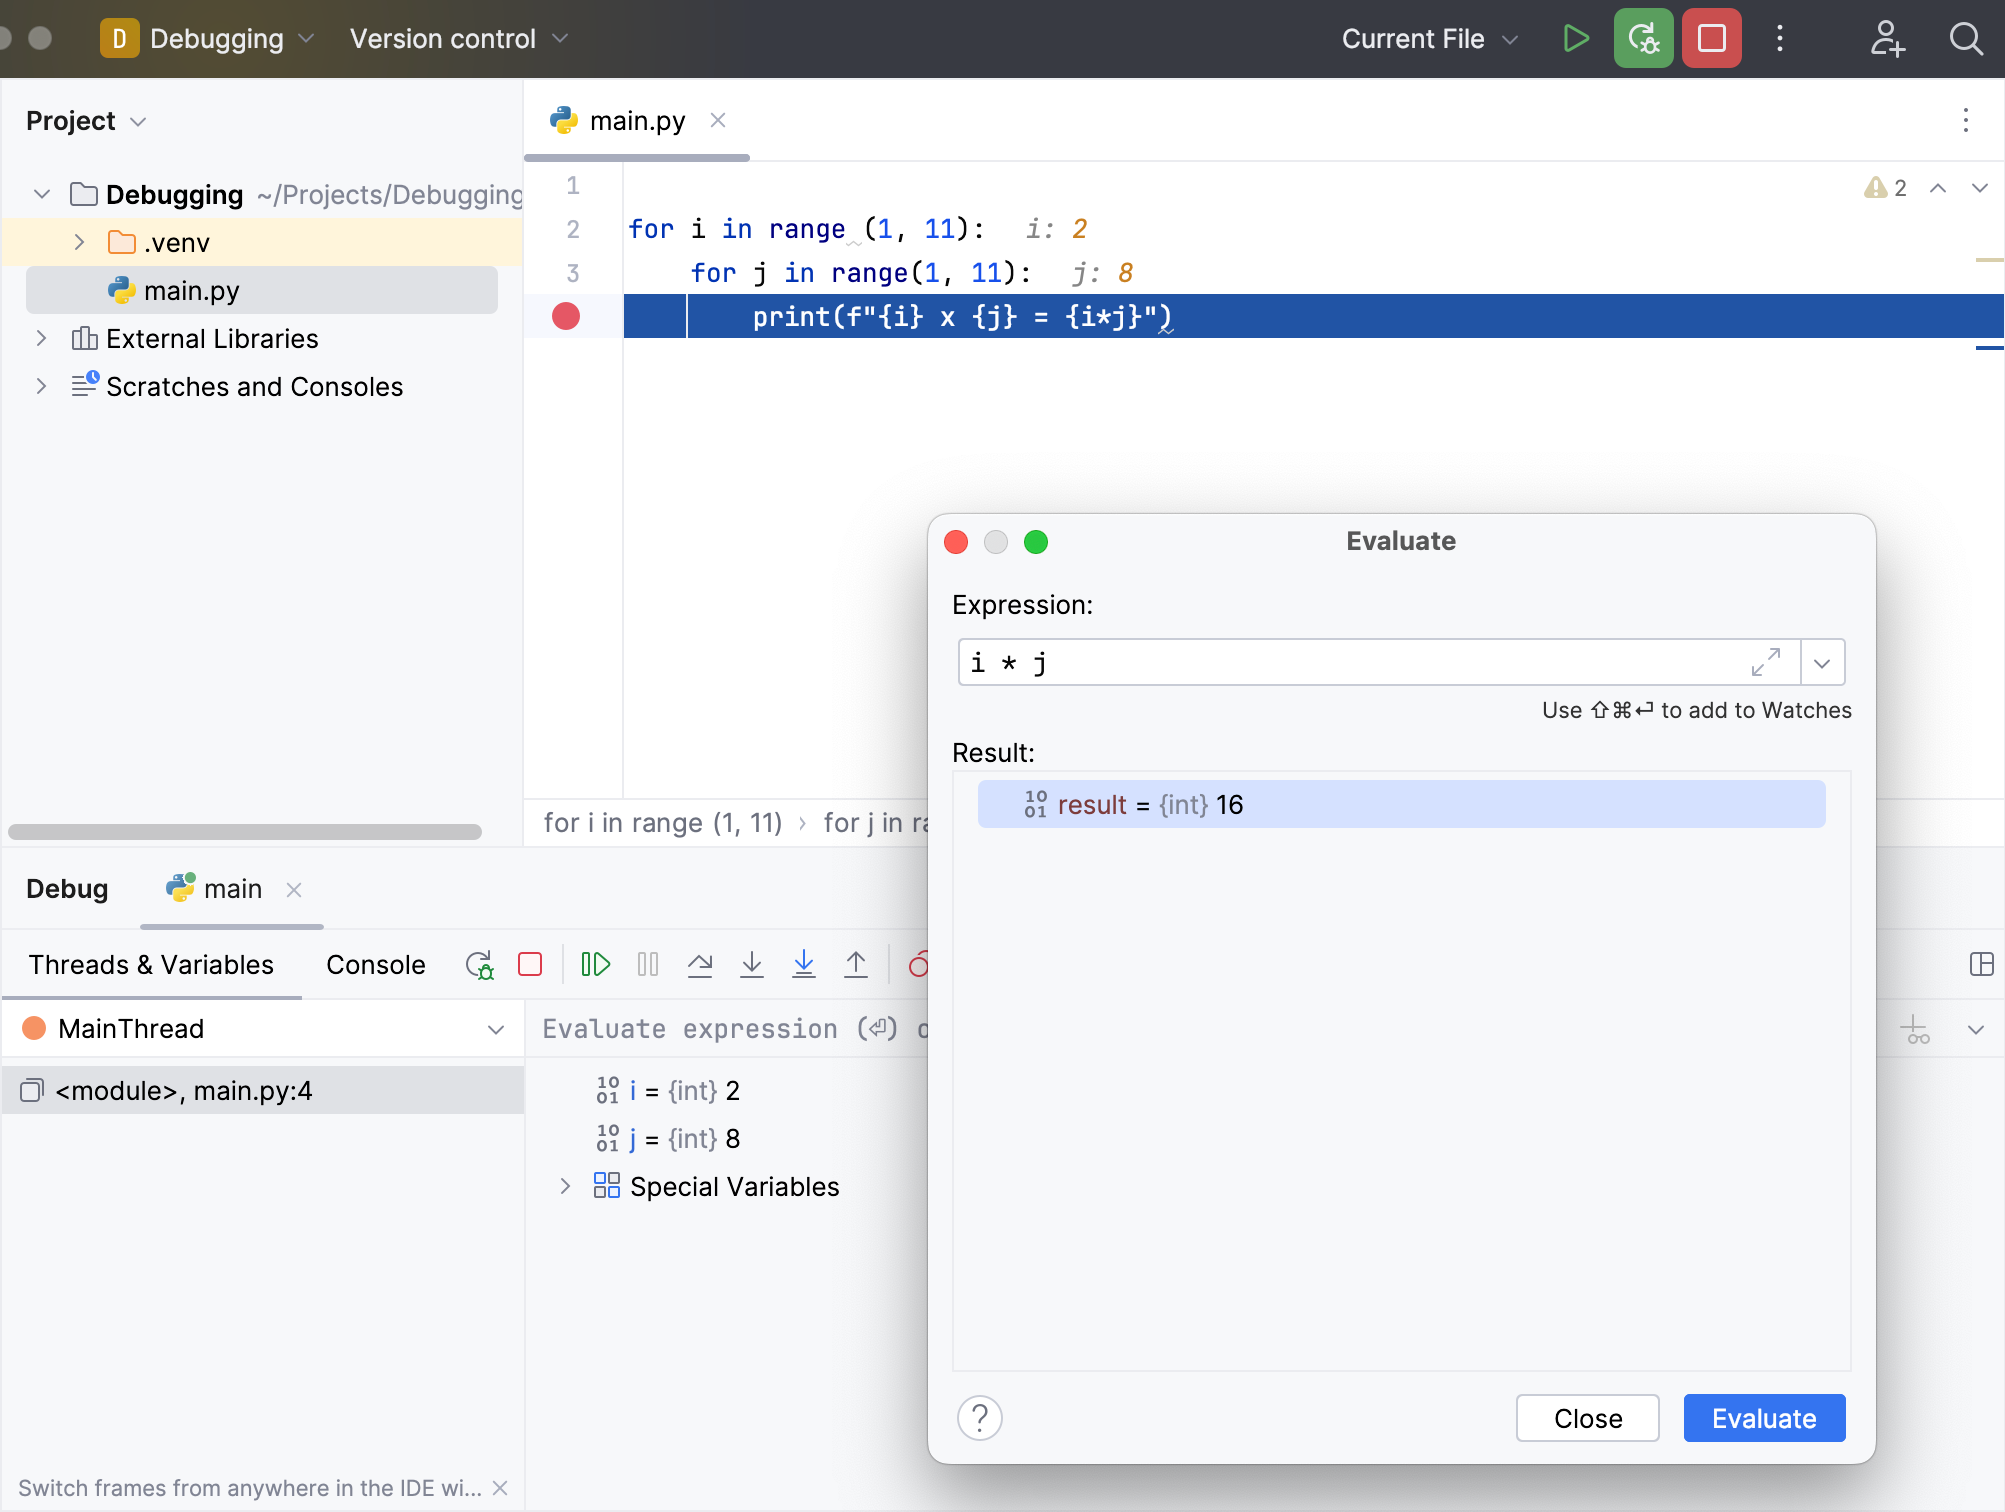
\includegraphics[width=\linewidth]{BreakPoint}
  \caption{
    \label{fig:breakpoint}
    Debugging a python program using breakpoint debugger and expression evaluation in PyCharm.
    }
\end{figure}

% \begin{figure}[hbt]
%   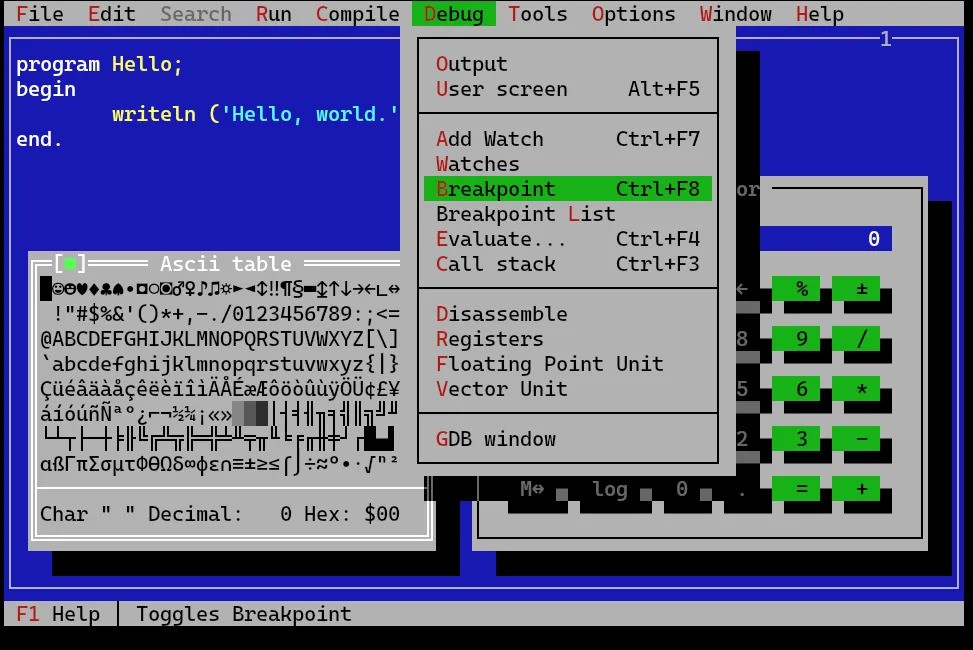
\includegraphics[width=\linewidth]{FreePascal.jpg}
%   \caption{
%     Run time debugging using break point in the Free Pascal interactive development environment in a command line window
%     }
% \end{figure}

% \begin{figure}[hbt]
%   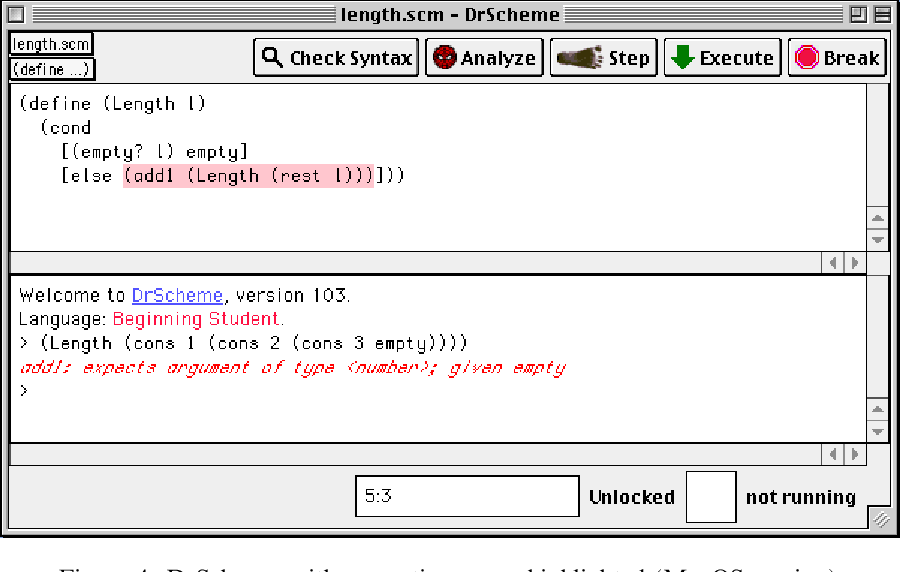
\includegraphics[width=\linewidth]{DrScheme}
%   \caption{
%     Dr Scheme, an interactive development environment for the Scheme language, highlights a runtime error
%     }
% \end{figure}

My research is motivated by the inherent difficulties in debugging type errors and the dormant development of improving type errors using modern graphical capabilities and HCI techniques.

\section{Research Aim}

\subsection{Aim 1. Provide Progremmers With The Comprehensive Knowledge Needed to Understand and Resolve Type Errors.}

To date, there is no unified representation of type errors. Most contemporary compiler tools represent type error as the combination of three pieces of information: a location where the type checking failed, an expected type, and the actually encountered type. We argue that this representation is far from being a helpful one. Thus we question that what is needed to comprehensively explain an type error. We try to address this question by careful examine the limitations of existing systems (\ref{sec:symptoms}) and the thought process of how programmers sovling type errors.

\subsubsection{Objective 1.1 To Encompass Multiple Potential Causes Of A Type Error}
One important focus of my work is to address the bias in traditional type errors (Section \ref{subsec:bias}). In this, we need to inform programmes that there always exist more than one possible causes of a type error, just as there are multiple ways to resolve the type error. To achieve this, the dimansion of potential causes is key information need to be defined, undestood, and exercised in practice.Each potential causes comprize a few key questions: what is the offending code, what are the resulting type assigments of each expressions after the offending code is fixed.

\subsubsection{Objective 1.2 To Accurately Report Relevant Locations Contributing to Type Errors.}
Traditional tools are limited to reporting a single location for type errors, which many researchers have addressed as an unhelpful limitation. Programmers are often unable to find a resolution at the reported location and are forced to expand their search without guidance. We want to improve this by reporting accurate locations relevant to the type of error.

\subsubsection{Objective 1.3 To Give Reasons And Support Of Human Understanding}
Type error does not end with a location in the source code. Programmers can still struggle to resolve a type error even after reaching the exact location of the culprits, failing to understand the logical explanation of the type error. Internally, type errors can be caused by mismatched types, unfulfilled type class constraints, or trying to construct infinite types. Externally, type errors can be caused by typos, outdated type annotation, incomplete implementation, too few or too many arguments in a function application, etc. Helping programmers find the cause or provide an accurate inference of what is the cause of the type error.


\subsection{Aim 2. Support Programmers To Type Errors Through Interactive Modern Programming Environments.}

We aim to integrate rich type error data into a modern, visual programming environment and workflow that allows programmers to work more efficiently with strongly typed languages. When humans are put in the middle, more information does not equal better comprehension. With enriched data representation, we want to deliver type errors to better support programmers’ comprehension and the chance for a successful resolution.

\subsubsection{Objective 2.1 Communicate The Key Concepts Of Type Errors Effectively Using Modern Programming Tools}

The concepts of type errors are traditionally displayed as text. These concepts include error locations, explanations of causes, and type signatures. We explore more intuitive techniques and media to communicate these concepts to better facilitate comprehension. For instance, using inline highlit to mark the locations directly in the source code provides better usability than printing the lines of interest in the terminal window.

\subsubsection{Objective 2.2 Use Interactive Tools for Investigating and Resolving Type Errors.}

To avoid presenting overwhelming information, we explore different techniques of interactively exploring the type errors. These techniques aim to divide the type error into smaller units that can still be assign meaning to, and provide a means for programmers to incrementally triangulate the potential root cause in the source code. This objective also involve provide situation aware debugging information, meaning that the error message should provide varying level of detail in the debugging information based on the context of the type error and progammers personal preference.


\section{Contributions}

\subsection{A categorization of type errors based on the structure of the evidence of a type error}

In order to illustate the challenges of providing comprehensive explanation of type errors, we divide the type errors into 3 categories. This categorization is based on how it is normally understood from human debugging perspective. It should be made clear that these categories are not mutually exclusive, a multi-witness type error can also be a multi-step type error at the same time.  

A \textbf{multi-step type error} is a type error that involves chain of based on the evidence of the type error. An typical multi-step type error is shown in the example (Fig \ref{fig:multi-step-example}). In the example, the chains of inference are the assigment of a (Line 1), the equivalence of a (Line 1 and line 2), the assigment  of b (Line 2) and the equivalence of b (Line 2 and Line 3). Removing any one of the chains will resolve the conflict. An important challenge with multi-step type errors is to convey this chain of infrence relation of relevant location. 

\begin{figure}[hbt]
  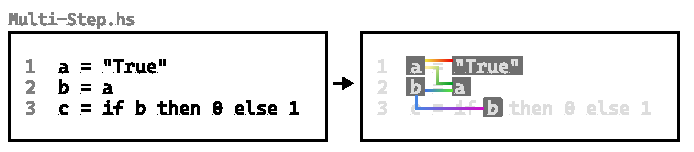
\includegraphics[width=\linewidth]{Multi-Step}
  \caption{
    \label{fig:multi-step-example}
    An example of multi-step type error.
    }
\end{figure}

A \textbf{multi-witness type error} is a type error that involves multiple piece of evidence supporting the same potential type assignments.  An typical multi-step type error is shown in the example (Fig \ref{fig:multi-witness-example}). In the example, multiple evidence (line 3,4,5) support that a has the type \texttt{Int -> String}. On the other hand, a single piece of evidence (line 2) show that a has the type \texttt{Int -> Char}  The challenge of presenting multi-witness type errors is to clearly show the opposing sides, and the number of witnesses of each side. 

\begin{figure}[hbt]
  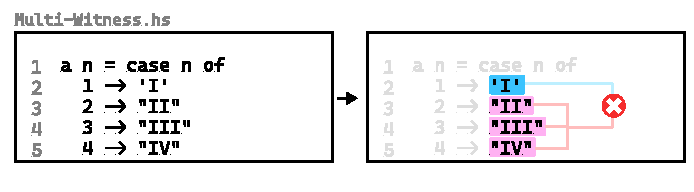
\includegraphics[width=\linewidth]{Multi-Witness}
  \caption{
    \label{fig:multi-witness-example}
    An example of multi-witness type error.
    }
\end{figure}

A \textbf{multi-party type error} is a type error that involves more than two typing possibilities.  An typical multi-step type error is shown in the example (Fig \ref{fig:multi-party-example}). In the example, the expression \texttt{d} can not be assign a type because 3 pieces of eveidence on line 1 suggesting 3 potential types for \texttt{d}. In pratice, multi-party type error is thought to be less intuitive and harder to properly explain. The most prominent task is to break down the type error into multiple simpler form of type errors. 



\begin{figure}[hbt]
  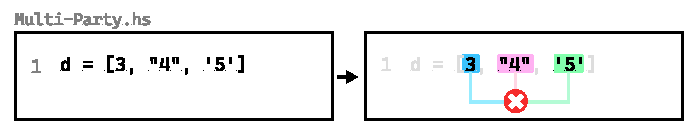
\includegraphics[width=\linewidth]{Multi-Party}
  \caption{
    \label{fig:multi-party-example}
    An example of multi-party type error.
    }
\end{figure}

With this classification, We contributed three systems -- Chameleon, Goanna and GeckoGraph -- each focusing on one or two unique challenges of type error debugging.

\subsection{Explaining Multi-Step Type Errors Through Chain-Of-Thought Visualization}

\subsubsection{Technical Contribution - Chameleon}
We contribute Chameleon, an interactive type error debugging tool for Haskell. Internally, Chameleon computes all relevant locations that contribute to the type of error. Via a set of iteratively designed interfaces, Chameleon preserves the two alternatives of the type error and the supporting evidence for each. Chameleon provides an unique debugging interface that allowing interactive explore the chain of reasoning in a multiple-step type error. In this interace, programmers see a pair of locations at a time, they are also shown how the two locations are logically related. This allow programmers to interactively developing a panaroma view of the type error. 

\subsubsection{An evaluation on the effect of error slicing and chain of thought visualizations}
We contributed a series of studies of the effects of debugging with visual representation of types and interactively explored type errors. We show that there is a difference between using traditional tools and enhanced type error debugging tools like Chameleon. And we show that this difference is more significant when debugging complex type errors.

\subsection{Iterate potential causes of multi-witness and multi-party errors}

\subsubsection{Technical Contribution -- Goanna}
We contribute Goanna, a type error debugging tool for Haskell. 
Similar to Chameleon, Goanna provide a compreseive set relevant locations that contribute to the type error and perseve the alternatives to the type error. 

However,  Goanna presents a type error by dividing it into a list of potential causes and their respective fixes. With Goanna, Haskell programmers can resolve type errors by exploring a list of potential root causes of errors. These causes are ordered using our heuristics so that the more likely causes are on top. 

\subsubsection{An evaluation on accuracy, conciseness, and performance of MCS-based type debugging and our heuristics}

We evaluated Goanna's effectiveness using 86 diverse Haskell programs from online discourse, demonstrating its ability to accurately identify and resolve type errors. Additionally, we present a collection of techniques and heuristics to enhance Goanna's suggestion-based error diagnosis and show their effectiveness from our evaluation.
We show that via our empirical evaluation, Goanna outperforms existing Haskell compilers when explaining the type error, with the slight disadvantage of an increased computation time.


\subsection{Visualizing Types}

\subsubsection{Technical Contribution -- GeckoGraph}

We contribute GeckoGraph, a graphic notation for Haskell types. GeckoGraph describes the same information as type signatures, but uses colors, shapes, and symbols to make certain structures easy to identify at a glance. GeckoGraph is designed to use visual elements to improve the understanding of type-level concepts, such type classes, parametric type variables, and high-rank types. When used to compare two types, GeckoGraph helps clarify differences visually. It makes errors like too few or too many arguments in applications and unmet type class constraints obvious.

\subsubsection{An evaluation on how programmers use graphic type notation}

We conducted a large-scale study on the effectiveness of using GeckoGraph to perform a series of Haskell tasks. We concluded that with GeckoGraph, programmers are more likely to succeed in programming tasks involving polymorphic types. The difference is more significant within less expereience programmers.

% \section{Research Method}

% \subsection{Human-centered programming language studies}

% One important decision that shape a lot of my work is employing human-centered research methods with our novel programming language systems. The adopting of human-centered methods happens at every stage of the projects: prototyping, development and evaluation. Although the using of these methods are not new at all, but they certainly are not the most polular choices in programming language studies.

% The motive of such decision is that it is impossible to understand what are the good qualities of type errors without observing how human use type errors to gain understanding. 


% The downside of study programming language is iterative design is very hard. programming tasks involves complex inputs and outputs, and it is very hard to study an incomplete system without a fully working systems. For instance, if we are to study the effect of type errors, it is most effective to have a system that can recognize type-correct program from ill-typed one. It is hard to evaluate with a mock-up or wizard of oz style fake outputs to study users' interaction.  To address this limitations, we have a few ideas implemented in our research:

% A minimal but practical set of language 
% Design for human from start



\section{Thesis outline}

The thesis can be divided into two parts. The first part (Chapters 1, 2) surveys the vivid panorama of type systems and programming languages. The purpose of these chapters is too situate the work  in later chapters, and to introduce the proper definitions and terminologies  used in this thesis.  The second part (Chapters 4, 5, 6, and 7) delves into three individual pieces of work, each targeting a uniqe problem in type error debugging.


\subsection{Chapter 2}
We provide some technical background in this chapter. This includes the traditional methods of Haskell type checking, type error slicing, interactive debugging. Following this direction, we continue to discuss the tools and techniques in constraint satisfiability analysis that we use in later chapters to improve type error reporting. Last, we revisit the categorization of type errors, provide a new way to define their meanings with the help of definitions we expored in chapter 2.


\subsection{Chapter 3}
This chapter introduces the work related to Chameleon and our study on its effect on debugging type errors. This chapter starts with an introduction of our motivation, succinctly summarised in three characteristics of bad-type error messages. We then introduce the key features Chamaleon, using the example of a  hypothetical programmers combating Haskell-type errors, luckily with the help of Chameleon. We go on to introduce the system design and iterative prototyping methods used to develop Chameleon. Lastly, we present our series of experiments on Chameleon's effect on solving type errors compared to traditional compiler tools. 


\subsection{Chapter 4}

In Chapter 5 we discuss our work: the Goanna type debugger and our evalution on its key aspects (accuracy, conciseness and performance). We first report some common limitations of traditional compiler error messages. We then go on to showcase some novel features of Goanna, including suggesting fixes, ranking causes by their likelyhood, type error isolation, and cross-module type error debugging.  Next, we discuss the implementation of Goanna and our heuristics for ranking potential causes and removing unhelpful suggestions. Last, we show our empirical study of the accuracy, conciseness, and performance of Goanna using a collection of real-world type errors in Haskell code. 

\subsection{Chapter 5}

In this chapter, we discuss our work on visualizing type annotations. In this, we showed GeckoGraph, a visual  language for haskell type. We also present our empirical study on how progrmmers use polymophic types and the effect of GeckoGraph. We start by presenting some usability challenges in using polymorphic types. We then describe the design goal of GeckoGraph and how it can be constructed from a textual type annotation using a few construction rules. We then show our large-scale study on the effect of using visual type annotations in programming and solving type errors. 


\subsection{Chapter 6}

In the last chapter, we reiterate our contributions with more remarks on their contexts. We discuss a few directions for future work. This includes the direction in future tool development, as well as future research opportunities. Lastly, in closing words, we return to the map field of programming language and the vast uncharted area of the future of programming. 